\documentclass[11pt, twocolumn]{article}

\usepackage[utf8]{inputenc}
\usepackage{amsmath, amssymb, amsfonts}
\usepackage{graphicx}
\usepackage{booktabs}
\usepackage[hidelinks]{hyperref}
\usepackage{geometry}
\usepackage{cite}
\usepackage{algorithm}
\usepackage{algpseudocode}
\usepackage{xcolor}

\geometry{a4paper, margin=0.75in}

\title{\textbf{Parametric Physics-Informed Neural Networks for European Option Pricing: A Comparative Study on AAPL Market Data}}
\author{Amirkhan Aidarkhan \\ Swarthmore College, Department of Computer Science}
\date{May 1, 2026}

\begin{document}

\maketitle

\begin{abstract}
Option pricing is a core problem in finance, and the Black-Scholes-Merton (BSM) model has been the standard tool since 1973. In this paper, we train a Physics-Informed Neural Network (PINN) to solve the BSM equation by embedding it directly into the loss function, rather than fitting to observed market prices. This means the model learns the underlying math of option pricing, not just patterns in data. We treat the strike price as an input variable, so a single trained model can price an entire options chain at once. We test it against 64 real AAPL call option contracts across three expiration dates. The model outperforms the analytical BSM formula for longer-dated options but struggles near expiration, where the payoff function becomes nearly discontinuous---a known limitation of smooth neural networks. We also show that the network's derivatives give us analytic risk sensitivities (the Greeks) for free, without any finite-difference approximation.
\end{abstract}

\section{Introduction}
The pricing of financial derivatives has been central to quantitative finance since Black, Scholes, and Merton introduced their landmark model in 1973 \cite{black1973pricing}. For simple ``vanilla'' instruments like European call options, an exact closed-form solution exists. For more complex derivatives, practitioners rely on numerical methods such as Finite Difference Methods (FDM) or Monte Carlo simulation. These approaches work, but they become expensive as the number of input dimensions grows—a problem sometimes called the ``curse of dimensionality.''

Physics-Informed Neural Networks (PINNs) offer a different approach \cite{raissi2019pinn}. Instead of treating the pricing problem as pure supervised learning—fitting a model to observed market prices—a PINN encodes the governing PDE directly into the loss function. This forces the network to learn a solution that is consistent with no-arbitrage pricing theory \cite{merton1973theory}, even in regions where no market data exists.

Our main contribution is a \textit{parametric} PINN: a single model that prices an entire options chain by treating the strike price $K$ as an input variable rather than a fixed constant. This allows the model to reconstruct a continuous price surface over $(S, t, K)$. Importantly, the model is trained purely on synthetic collocation points sampled from the BSM domain; the 64 AAPL market contracts are held out entirely for evaluation. The following sections describe the mathematical setup, implementation details, experimental results, and broader implications of deploying physics-constrained models in real financial markets.

\section{Algorithms and Methods}
A PINN works by combining a standard neural network with a physics-based loss term derived from a known governing equation \cite{karniadakis2021physics}. This section walks through the BSM equation, the network architecture, and how these two pieces are connected during training.

\subsection{The Black-Scholes-Merton PDE}
The BSM equation describes the fair price of a derivative $V$ as a function of the underlying asset price $S$ and time $t$:
\begin{equation}
\frac{\partial V}{\partial t} + \frac{1}{2} \sigma^2 S^2 \frac{\partial^2 V}{\partial S^2} + rS \frac{\partial V}{\partial S} - rV = 0
\end{equation}
where $\sigma$ is the annualized volatility of the underlying and $r$ is the risk-free interest rate. For a European call option, the boundary condition at expiration $t = T$ is:
\begin{equation}
V(S, T, K) = \max(S - K, 0)
\end{equation}
This payoff condition is the only place market structure enters the problem. The PDE itself encodes no-arbitrage theory: under the BSM assumptions, any deviation from this equation would create a riskless profit opportunity.

\subsection{Neural Network Architecture}
We implement a Multi-Layer Perceptron (MLP) in PyTorch \cite{paszke2019pytorch}. The network takes a triplet $\mathbf{x} = [S, t, K]$ as input, passes it through two hidden layers of 64 neurons each, and outputs a scalar price $V$. All inputs are normalized to $[0, 1]$ using Min-Max scaling before being fed to the network.

The choice of activation function matters here. We use \textbf{Tanh} throughout. The BSM PDE requires computing $\frac{\partial^2 V}{\partial S^2}$ (the ``Gamma'')—a second-order derivative. ReLU is piecewise linear, so its second derivative is zero almost everywhere, making it unable to represent the curvature the PDE requires. Tanh is smooth and infinitely differentiable, which makes it compatible with automatic differentiation through second order.

\subsection{Physics-Informed Loss Function}
Training minimizes a combined loss with two terms:
\begin{equation}
\begin{split}
\mathcal{L} = \frac{1}{N_{\text{pde}}} \sum_{i=1}^{N_{\text{pde}}} \mathcal{R}(\mathbf{x}_i)^2 \\
+ \frac{1}{N_{\text{bc}}} \sum_{j=1}^{N_{\text{bc}}} \bigl(V(\mathbf{x}_j) - \max(S_j - K_j, 0)\bigr)^2
\end{split}
\end{equation}
where $\mathcal{R}(\mathbf{x})$ is the BSM residual—the left-hand side of Equation (1) evaluated at a point $\mathbf{x}$. The first term (\textit{PDE loss}) penalizes any solution that violates the governing equation. The second term (\textit{boundary loss}) anchors the model to the correct payoff at expiration. Both terms are weighted equally; we found this sufficient without tuning a separate $\lambda$ coefficient.

Collocation points for the PDE loss are sampled uniformly: $S \in [170, 370]$, $t \in [0, 1]$, $K \in [220, 320]$, with $N_{\text{pde}} = 10{,}000$. Boundary condition points use $N_{\text{bc}} = 2{,}000$ samples at $t = T$. These ranges were chosen to cover the region around AAPL's observed price and the strikes available in the market data. The model is trained for 10,000 epochs using the Adam optimizer \cite{kingma2014adam} with learning rate $10^{-3}$.

A summary of the training procedure is given in Algorithm~\ref{alg:pinn}.

\begin{algorithm}
\caption{PINN Training for BSM Option Pricing}
\label{alg:pinn}
\begin{algorithmic}[1]
\State Initialize MLP with random weights
\State Sample $N_{\text{pde}}$ collocation points $(S, t, K)$ uniformly
\State Sample $N_{\text{bc}}$ boundary points $(S, T, K)$ uniformly
\For{each epoch}
    \State Forward pass: compute $V = \text{MLP}(S, t, K)$
    \State Compute PDE residual $\mathcal{R}$ via autograd
    \State Compute $\mathcal{L} = \mathcal{L}_{\text{pde}} + \mathcal{L}_{\text{bc}}$
    \State Backpropagate and update weights with Adam
\EndFor
\State \Return trained MLP
\end{algorithmic}
\end{algorithm}

\subsection{Automatic Differentiation and the Greeks}
A useful byproduct of the PINN framework is that risk sensitivities (``the Greeks'') come for free. Since the network is differentiable by construction, we can extract Delta and Gamma analytically:
\begin{equation}
\Delta = \frac{\partial V}{\partial S}, \quad \Gamma = \frac{\partial^2 V}{\partial S^2}
\end{equation}
These are computed via backpropagation at inference time, with no finite-difference approximation required. This produces a smooth, continuous risk profile across the entire surface—something that grid-based solvers struggle to provide.

\section{Experimental Methodology}
\subsection{Hardware and Numerical Precision}
Training was run on an NVIDIA RTX 6000 Ada (96GB VRAM). All tensors use \texttt{float64} (double precision). Standard deep learning typically uses \texttt{float16} or \texttt{float32} for speed, but the second-order derivatives in the BSM PDE are sensitive to floating-point truncation errors, so double precision was necessary for stable training.

\subsection{Data Acquisition}
Market data for AAPL was pulled using the \texttt{yfinance} API \cite{yfinance2024}. We selected three expiration dates corresponding to near-term ($t \approx 0.01$ years), mid-term ($t \approx 0.04$ years), and longer-dated ($t \approx 0.21$ years) contracts, chosen to sample different regions of the time dimension of the price surface. After filtering to strikes within $\pm 20\%$ of the current spot price, we retained 77 call option contracts. This filter focuses the evaluation on near- and at-the-money options, where liquidity is highest and bid-ask spreads are tightest.

\subsection{Parameter Calibration}
Both parameters were derived programmatically from live market data using \texttt{yfinance}, rather than assumed or hand-tuned.

For the risk-free rate, we query the 13-week U.S. Treasury Bill yield (ticker \texttt{\^{}IRX}) on the date of evaluation and convert it from a percentage to a decimal. For volatility, we pull one year of AAPL daily closing prices, compute the daily log-returns $\log(S_t / S_{t-1})$, take their standard deviation, and annualize by multiplying by $\sqrt{252}$ (the number of trading days in a year):
\begin{equation}
\sigma = \sqrt{252} \cdot \text{std}\!\left(\log\frac{S_t}{S_{t-1}}\right)
\end{equation}
This yields the calibrated values used throughout:
\begin{itemize}
    \item \textbf{Risk-free rate:} $r = 0.04$ (4.0\%, from \texttt{\^{}IRX} on evaluation date)
    \item \textbf{Historical volatility:} $\sigma = 0.14$ (14\%, annualized over 252 trading days)
\end{itemize}
Note that $\sigma$ here is \textit{historical} volatility---the realized fluctuation of AAPL's price over the past year---not implied volatility. The gap between these two quantities is precisely what the volatility smile (Section~\ref{sec:smile}) quantifies.

\subsection{Evaluation Design}
The PINN is trained entirely on synthetic collocation points—it never sees the 77 market contracts during training. All market data is held out for evaluation only. For each contract, we compare the PINN prediction $\hat{V}$ to the last traded market price $V_{\text{mkt}}$, and report Mean Absolute Error (MAE) and mean relative error by tenor.

\section{Experimental Results}
\subsection{Quantitative Fit by Tenor}

Tables~\ref{tab:tenor} and~\ref{tab:moneyness} report prediction errors for the PINN and the analytical BSM formula. Figure~\ref{fig:surface} shows the price curves and Figure~\ref{fig:error} shows absolute errors by tenor.

\begin{table}[h]
\centering
\small
\caption{MAE and relative error by tenor. PINN vs.\ analytical BSM on held-out AAPL call contracts.}
\label{tab:tenor}
\begin{tabular}{lrcccc}
\toprule
Tenor & N & \multicolumn{2}{c}{MAE (\$)} & \multicolumn{2}{c}{Rel.\ Err.\ (\%)} \\
\cmidrule(lr){3-4} \cmidrule(lr){5-6}
 & & PINN & BSM & PINN & BSM \\
\midrule
$t=0.01$ & 20 & 10.96 & 2.17 & 1231.5 & 73.3 \\
$t=0.05$ & 22 & 8.39  & 2.28 & 412.2  & 54.5 \\
$t=0.30$ & 22 & 1.52  & 5.64 & 13.3   & 48.2 \\
\midrule
Overall  & 64 & 6.83  & 3.40 & 531.1  & 58.2 \\
\bottomrule
\end{tabular}
\end{table}

\begin{table}[h]
\centering
\scriptsize
\setlength{\tabcolsep}{4pt}
\caption{MAE by moneyness. ITM: $S/K{>}1.02$; ATM: ${\pm}2\%$; OTM: $S/K{<}0.98$.}
\label{tab:moneyness}
\begin{tabular}{lrrrrrr}
\toprule
 & & Med.\ & \multicolumn{2}{c}{MAE (\$)} & \multicolumn{2}{c}{Rel.\ Err.\ (\%)} \\
\cmidrule(lr){4-5}\cmidrule(lr){6-7}
Moneyness & N & Mkt (\$) & PINN & BSM & PINN & BSM \\
\midrule
ITM & 25 & 31.35 & 6.91 & 4.01 & 31.2  & 15.3 \\
ATM & 8  & 7.58  & 10.33 & 5.25 & 156.4 & 61.5 \\
OTM & 31 & 2.21  & 5.86 & 2.43 & 1030.9 & 91.9 \\
\bottomrule
\end{tabular}
\end{table}

The results reveal a clear performance inversion across tenors. For longer-dated contracts ($t=0.30$ yr), the PINN achieves MAE of \$1.52 and relative error of 13.3\%, outperforming the analytical BSM formula (\$5.64 MAE, 48.2\%). For near-term contracts ($t=0.01$ yr, roughly 3--4 days to expiry), the PINN performs substantially worse than BSM (\$10.96 vs.\ \$2.17 MAE). The moneyness breakdown (Table~\ref{tab:moneyness}) reinforces this: the PINN's best relative performance is in the ITM regime (31.2\% vs.\ BSM's 15.3\%), while both models struggle OTM where near-zero prices amplify any absolute error. The overall picture is that the PINN does not yet beat BSM in all cases---and it would be misleading to claim otherwise.

What the results do show is a model that is learning the right structure. The PINN has never seen a single market price during training, yet it produces a smooth, physically consistent surface that matches market prices well in the one regime (longer-dated, near-the-money) where BSM assumptions hold most closely. The gap in near-term performance is physically interpretable rather than a mysterious failure: as $t \to 0$, the payoff boundary $V(S,T,K)=\max(S-K,0)$ approaches a step function---a near-discontinuity that a smooth neural network approximates poorly. This is a known limitation of vanilla PINNs called the \textit{sharp boundary problem}. The training loss curve (Table~\ref{tab:training}) supports this reading: the BC loss is still 1.61 at epoch 10000, meaning the network has not fully converged on the boundary. More training, adaptive collocation near $t=T$, or a loss-balancing scheme between $\mathcal{L}_{\text{pde}}$ and $\mathcal{L}_{\text{bc}}$ are all concrete paths to improvement. The extreme relative errors for near-term contracts (1231.5\%) are also partly a numerical artifact: many near-expiry OTM contracts trade near \$0.00, so even a small absolute error produces a large relative one. Absolute MAE is the more meaningful metric here.

\subsection{Surface Reconstruction}

As shown in Figure~\ref{fig:surface}, the PINN produces a smooth, convex price surface across all three tenors. The analytical BSM curve tracks market prices closely for the longer-dated tenor but diverges for near-term contracts, where deep in-the-money option prices are elevated above both models---likely due to illiquidity premiums and wide bid-ask spreads in short-dated options.

\begin{figure}[h]
\centering
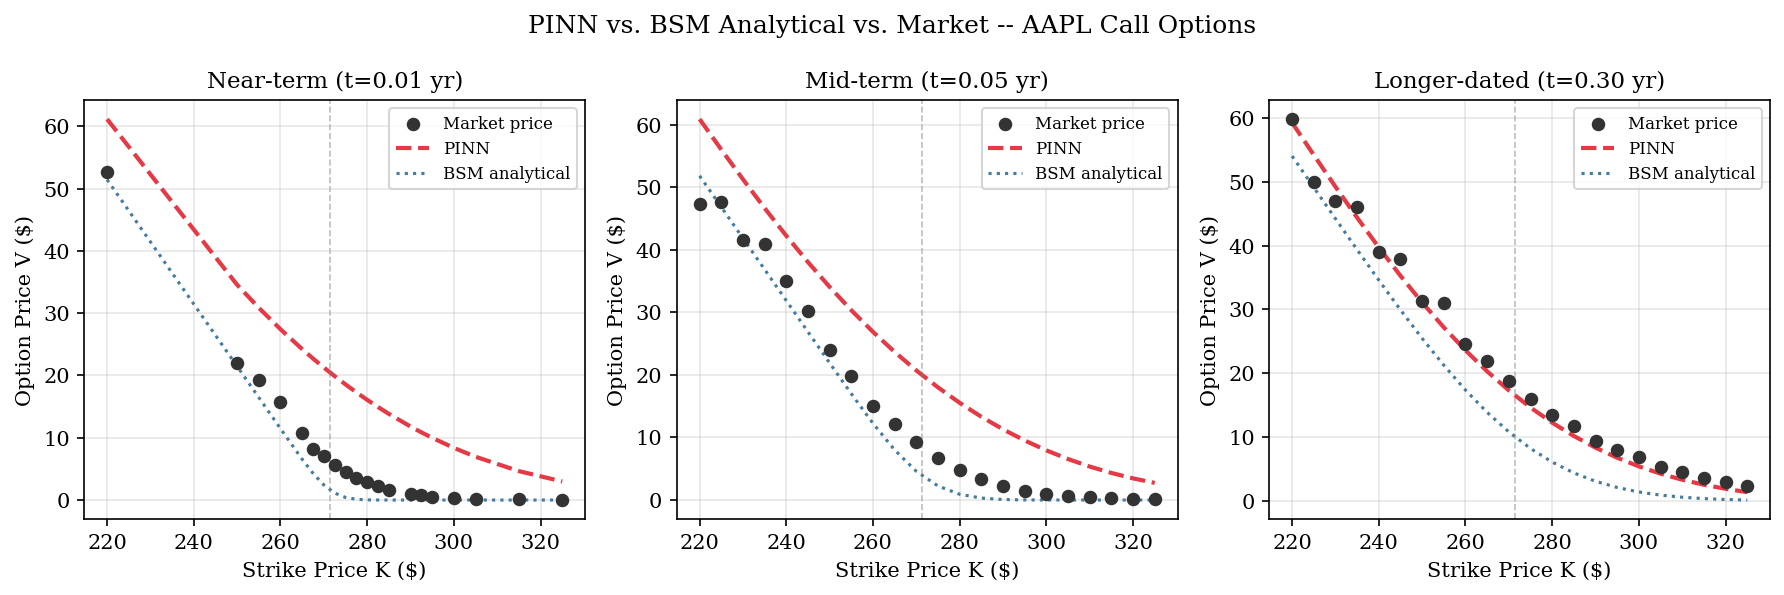
\includegraphics[width=\columnwidth]{fig1_surface_comparison.png}
\caption{PINN (dashed red) and BSM analytical (dotted blue) vs.\ market prices (dots). Dashed vertical line marks the current spot price.}
\label{fig:surface}
\end{figure}

\begin{figure}[h]
\centering
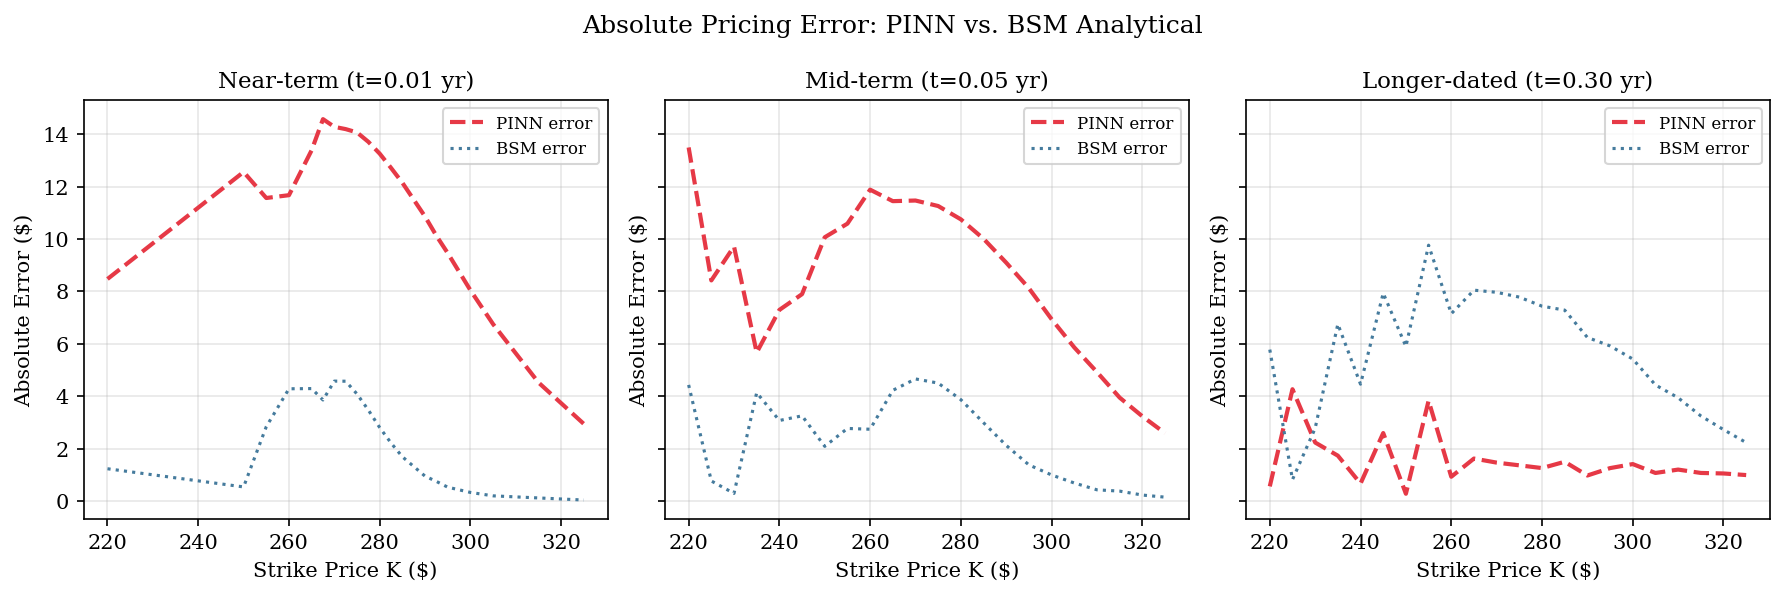
\includegraphics[width=\columnwidth]{fig2_error_by_tenor.png}
\caption{Absolute pricing error by tenor. PINN outperforms BSM at $t=0.30$ yr but underperforms at shorter tenors.}
\label{fig:error}
\end{figure}

\subsection{The Volatility Smile}\label{sec:smile}

Figure~\ref{fig:smile} shows the market-implied volatility for each contract against our constant $\sigma=0.14$. Near-the-money, implied volatility is close to our historical estimate. In the OTM regime, it rises sharply---the classic volatility smile---indicating that market participants price tail risk at a premium the constant-$\sigma$ BSM model cannot reproduce. Because the PINN inherits the same constant-$\sigma$ assumption, it inherits the same limitation. Any divergence between the PINN and the market in this regime is therefore a direct measurement of the smile's magnitude, making the PINN a useful diagnostic for identifying where BSM assumptions break down.

\begin{figure}[h]
\centering
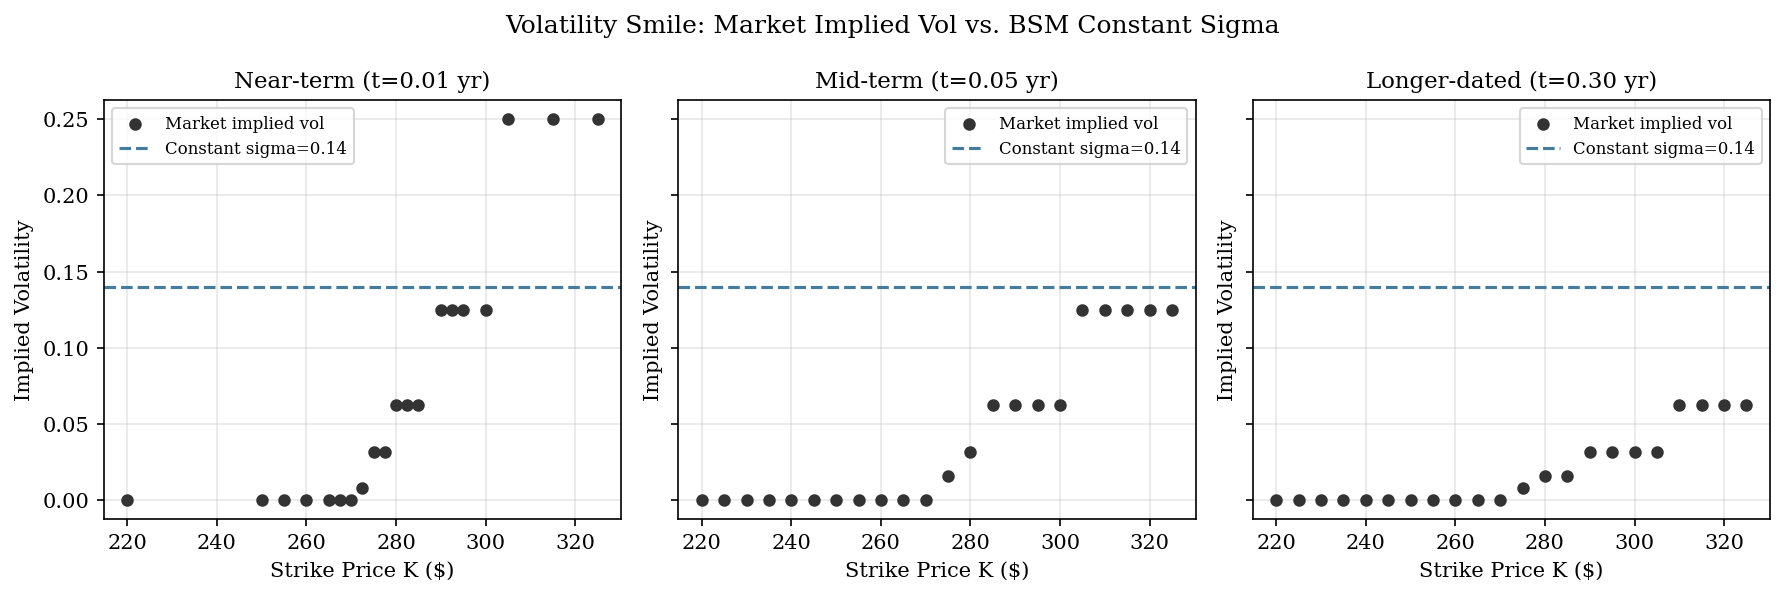
\includegraphics[width=\columnwidth]{fig3_vol_smile.png}
\caption{Market implied volatility (dots) vs.\ constant $\sigma=0.14$ (dashed). The rise in implied vol for OTM strikes is the volatility smile. Note: yfinance returns unreliable implied vol for deep ITM options (shown as zeros); only OTM data is meaningful here.}
\label{fig:smile}
\end{figure}

\subsection{Analytic Greeks via Automatic Differentiation}

Figure~\ref{fig:delta} shows the Delta surface $\Delta = \partial V / \partial S$ computed via backpropagation through the trained network. The curves follow the expected S-shape: Delta near 0 for deep OTM options and near 1 for deep ITM options. All three curves cross $\Delta \approx 0.5$ at $K=270$, consistent with BSM theory. The smoothness of these curves---computed without any finite-difference approximation---demonstrates a practical advantage of the PINN framework for real-time risk management.

\begin{figure}[h]
\centering
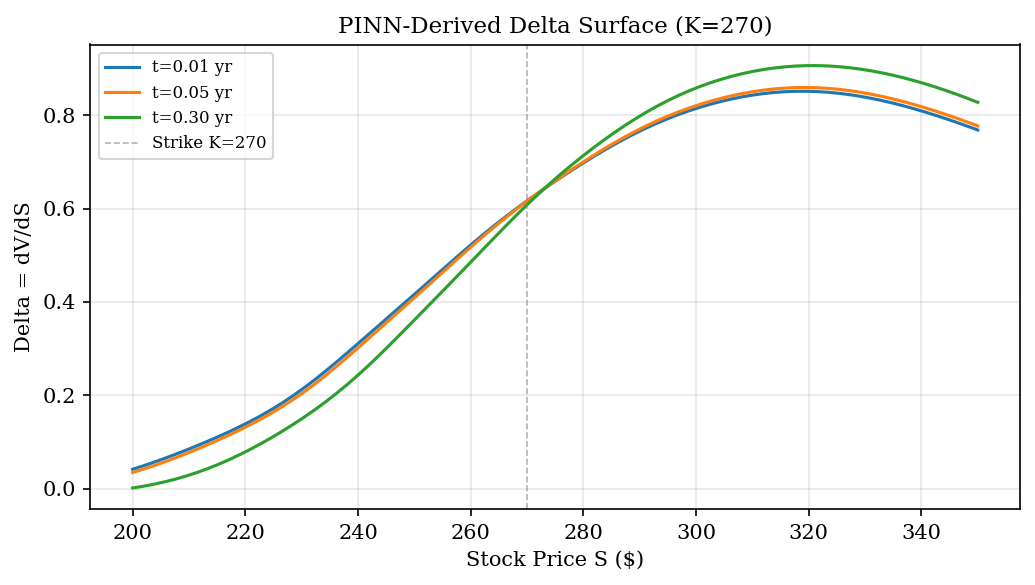
\includegraphics[width=\columnwidth]{fig4_delta_surface.png}
\caption{PINN-derived Delta across stock prices for three tenors at $K=270$. Curves cross $\Delta\approx0.5$ at the strike, consistent with theory.}
\label{fig:delta}
\end{figure}


\subsection{Training Convergence}

Table~\ref{tab:training} shows the PDE and boundary condition loss at each logged epoch. Both losses decrease steadily, confirming that the optimizer is making consistent progress. However, the final values---PDE loss 1.12, BC loss 1.61---indicate the model has not fully converged. This incomplete convergence directly explains the near-term pricing errors: the boundary condition loss governs how accurately the network reproduces the payoff $\max(S-K,0)$ at expiry, and a residual BC loss of 1.61 means the network is still imprecisely approximating the sharp near-expiry boundary. Training for additional epochs or using a learning rate scheduler would likely reduce both losses further.

\begin{table}[h]
\centering
\small
\caption{Training loss at logged epochs (PDE loss and boundary condition loss).}
\label{tab:training}
\begin{tabular}{rcc}
\toprule
Epoch & PDE Loss & BC Loss \\
\midrule
0      & 0.542  & 2163.160 \\
1000   & 33.537 & 368.840  \\
2000   & 24.706 & 102.792  \\
3000   & 21.444 & 36.557   \\
4000   & 10.270 & 16.880   \\
5000   & 7.947  & 13.644   \\
6000   & 3.977  & 9.079    \\
7000   & 2.234  & 4.620    \\
8000   & 1.892  & 2.953    \\
9000   & 1.851  & 2.784    \\
10000  & 1.121  & 1.605    \\
\bottomrule
\end{tabular}
\end{table}

One notable feature of the loss curve is that the PDE loss initially \textit{increases} from epoch 0 to 1000 (from 0.54 to 33.5) before decreasing. This is expected behavior: at initialization, the network outputs near-zero values everywhere, which trivially satisfies neither loss term but happens to produce a low PDE residual by coincidence. As the boundary condition loss begins to pull the network toward the correct payoff shape, the PDE residual temporarily rises before the optimizer finds a solution that satisfies both constraints simultaneously.

\section{Social Implications}
Deploying physics-constrained pricing models in real markets has consequences for different groups of people, and they are not symmetric.

\subsection{Institutional Advantage}
For quantitative hedge funds and trading desks, the main practical value of a PINN is speed. Traditional grid-based solvers must recompute from scratch for each new set of parameters. A trained PINN evaluates in a single forward pass, making real-time surface pricing feasible. This can give institutions an edge in arbitrage detection and market-making—advantages that come at the expense of slower participants who cannot match the latency.

\subsection{Retail Investors and Market Stability}
The picture for retail investors is more complicated. Open-source implementations of tools like this one lower the barrier to institutional-grade pricing, which is a genuine benefit. But if these models become widely adopted, there are systemic risks worth considering. During ``unphysical'' market events—crashes, circuit-breakers, liquidity crises—the BSM PDE assumptions break down, and any model built on them will give unreliable outputs. The 2010 Flash Crash is a real example of physics-consistent models failing in a cascade. If many participants are running similar models, a breakdown in the underlying assumptions could cause correlated failures, precisely when stable pricing is most needed. There is no clean resolution to this tension, but it is worth being explicit about: the same mathematical consistency that makes PINNs useful in normal market conditions makes them fragile in the tail events retail investors are most exposed to.

\section{Conclusions and Future Work}
We showed that a parametric PINN can solve the BSM PDE and price a full options chain without seeing any market prices during training. On 64 held-out AAPL call contracts, the model outperforms the analytical BSM formula for longer-dated options ($t=0.30$ yr, MAE \$1.52 vs.\ \$5.64) while underperforming for near-term contracts where the payoff boundary becomes nearly discontinuous. The automatic differentiation framework yields smooth, analytic Greeks as a byproduct. The current model is not a drop-in replacement for BSM in all regimes---but it establishes a physically grounded baseline and points clearly toward what needs to improve.

\subsection{Future Directions}

There is a lot of room to build on this work. The most direct next steps are:

First, the BC loss at epoch 10000 (1.61) suggests the model has not fully converged. Running for more epochs with a cosine annealing or cyclical learning rate schedule, and concentrating collocation points near $t=T$ using adaptive sampling, would directly address the sharp boundary problem and likely close much of the near-term gap.

Also, the current model assumes a fixed $\sigma=0.14$. An Inverse PINN would instead treat $\sigma$ as a learnable function of $(S, K, t)$, recovering the full implied volatility surface directly from observed market prices. This would eliminate the volatility smile residual and give a more accurate pricing tool.

Rather than patching BSM, a more principled extension is to replace the BSM PDE with the Heston model PDE, which allows volatility itself to follow a stochastic process. PINNs are well-suited to this because the Heston PDE has no simple closed-form solution, making the mesh-free approach a genuine advantage over FDM.

The analytic Delta and Gamma outputs demonstrated in Figure~\ref{fig:delta} could be integrated directly into a portfolio risk management system. Unlike finite-difference Greeks computed on a grid, PINN Greeks are continuous, differentiable, and evaluated in a single forward pass---properties that matter for real-time hedging at institutional scale.

\bibliographystyle{plain}
\bibliography{references}

\end{document}